In the early days of computing, programming was hard. The processors were slow, the memory was limited, the compilers were primitive, and nothing could be achieved without a major effort. The programmer had to know the architecture of the CPU, the layout of the memory, and when the compiler did not cut it, the critical code had to be written in assembler.

Then things got better. The processors were getting faster every year, the number that used to be the capacity of a huge hard drive became the size of the main memory in an average PC, and the compiler writers learned a few tricks to make programs faster. The programmers could spend more time actually solving problems. This was reflected in the programming languages and design styles: between the higher-level languages and evolving design and programming practices, the programmers' focus shifted from what they wanted to say in code to how they wanted to say it.

Formerly common knowledge, such as exactly how many registers the CPU has and what their names are, became esoteric, arcane matter. A "large code base" used to be one that needed both hands to lift the card deck; now, it was one that taxed the capacity of the version control system. There was hardly ever a need to write code specialized for a particular processor or a memory system, and portable code became the norm.

As for assembler, it was actually difficult to outperform the compiler-generated code, a task well out of reach for most programmers. For many applications, and those writing them, there was "enough performance," and other aspects of the programmers' trade became more important (to be clear, the fact that the programmers could focus on the readability of their code without worrying whether adding a function with a meaningful name would make the program unacceptably slow was a good thing).

Then, and rather suddenly, the free lunch of "performance taking care of itself " was over. The seemingly unstoppable progress of the ever-growing computing power just … stopped.


\hspace*{\fill} \\ %插入空行
\begin{center}
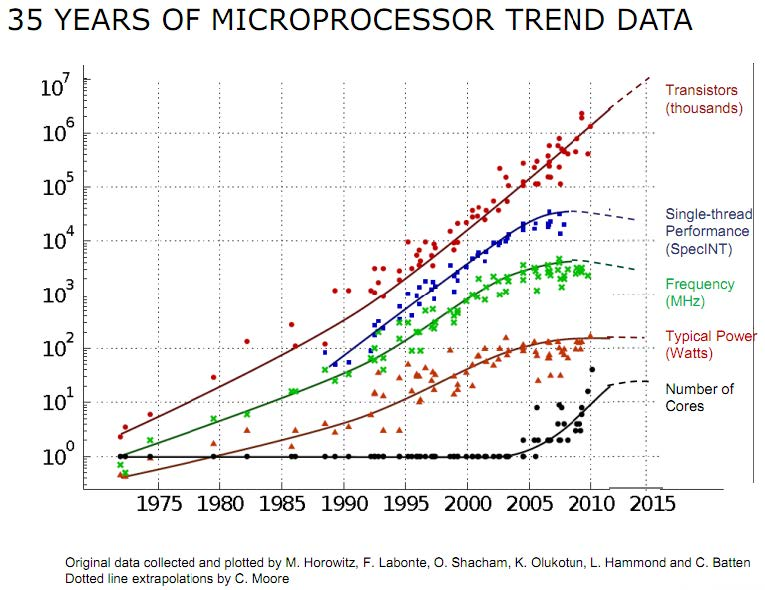
\includegraphics[width=0.9\textwidth]{content/1/chapter1/images/1.jpg}\\
Figure 1.1 – Charting 35 years of microprocessor evolution \\
(Refer to \url{https://github.com/karlrupp/microprocessor-trend-data and https://github.com/karlrupp/microprocessor-trend-data/blob/master/LICENSE.txt})
\end{center}

Around the year 2005, the computing power of a single CPU reached saturation. To a large extent, this was directly related to the CPU frequency, which also stopped growing. The frequency, in turn, was limited by several factors, one of which was power consumption (if the frequency trend continued unchanged, today's CPUs would pack more power per square millimeter than the great jet engines that lift rockets into space).

It is evident from the preceding figure that not every measure of progress stalled in 2005: the number of transistors packed into a single chip kept growing. So, what were they doing if not making chips faster? The answer is two-fold, and part of it is revealed by the bottom curve: instead of making the single processor larger, the designers had to settle for putting several processor cores on the same die. The computing power of all these cores together, of course, increased with the number of cores, but only if the programmer knew how to use them. The second part of the "great transistor mystery" (where do all the transistors go?) is that they went into various very advanced enhancements to the processor capabilities, enhancements that can be used to improve performance, but again, only if the programmer makes an effort to use them.

The change in the progress of processors that we have just seen is often held as the reason that concurrent programming has entered the mainstream. But the change was even more profound than that. You will learn throughout this book how, in order to obtain the best performance, the programmer once again needs to understand the intricacies of the processor and memory architecture and their interactions. Great performance doesn't "just happen" anymore. At the same time, the progress we have made in writing code that clearly expresses what needs to be done, rather than how it's done, is not to be rolled back. We still want to write readable and maintainable code, and (and not but) we want it to be efficient as well.

To be sure, for many applications there is still enough performance in modern CPUs, but performance is getting more attention than it used to, in large part because of the change in CPU development we just discussed and because we want to do more computing in more applications that do not necessarily have access to the best computing resources (for example, a portable medical device today may have a full neural network in it).

Fortunately, we do not have to rediscover some lost art of performance by digging through piles of decaying punch cards in a dark storage room. At any time, there were still hard problems, and the phrase there is never enough computing power was true for many programmers. As computing power grew exponentially, so did the demands on it. The art of extreme performance was kept alive in those few domains that needed it. An example of one such domain may be instructive and inspiring at this point.











